\section{Industrial Case Study}
Plasma etching \cite{Plummer2000} is an unit operations commonly used in semiconductor manufacturing. Figure~\ref{fig:plasma_etcher} shows a schematic of a plasma etch reactor.
Ionized etchant gases (usually fluorine, chlorine based, halide containing species)
reacts physio-chemically with the surface silicon. Figure~\ref{fig:plasma_etch} illustrates the different etching mechanisms that are simultaneously present. Isotropic etching could cause undercutting, while physical sputtering could cause trenching; both of which are undesirable
outcomes. To mitigate these effects, the trim time for the etch step has to
be controlled precisely, which requires an accurate process model.

In gate etching processes, line-width profiles and critical dimension are
critical parameters that correlate to the performance of the final device.
Metrology stations are used to measure these quality parameters before and
after gate etch to ensure wafer quality. These metrology measurements are
illustrated in Figure~\ref{fig:metrology_examples}.

\begin{figure}[!htpb]
  \centering
  \includegraphics[width=0.9\textwidth]{figures/intro/plasma_etcher.png}\\
  \caption{Schematic of a typical plasma etching system}
  \label{fig:plasma_etcher}
\end{figure}

\begin{figure}[!htpb]
  \centering
  \includegraphics[width=0.8\textwidth]{figures/intro/plasma_etch.png}\\
  \caption{Summary of etching mechanisms and typical problems in plasma etching}
  \label{fig:plasma_etch}
\end{figure}


\index{Gate etch}%
\index{FICD}%
\index{FICD!Final Inspection Critical Dimension}%
\index{DICD}%
\index{DICD!Develop Inspection Critical Dimension}%


\begin{figure}[!htpb]
  \centering
  \includegraphics[width=0.8\textwidth]{figures/application/metrology_meas.png}\\
  \caption{Transmission Electron Micrograph (TEM) of a polysilicon gate geometry showing the quality variables of interest}\label{fig:metrology_examples}
\end{figure}

The gate etch dataset contains 1800 wafers with metrology measurements of Develop-Inspect Critical Dimension of the resist pattern (DICD) and Final Inspect Critical Dimension
(FICD). Modeled outputs could be expressed as either the difference between
these measurements (etch bias) or the etch bias divided by the trim etch time
as the etch rate. This study attempts to predict the etch rate from the various process inputs of the etch tool. Figure~\ref{fig:raw_data_3} shows the etch rate of the entire dataset.
The first 205 wafers are used as training data; the rest of the dataset
are used for validation and testing.

The process inputs are collected through the fault detection and classification (FDC) system of the tool. 
The FDC measurements contain instrument read-outs from the RF circuitry, etchant gas flow
, chamber temperature, vacuum systems, and various spectroscopic sensors. The data collection rate is 0.5 Hz. Additional contexet information such as recipe step, process
time and EWMA-estimated disturbances in the controller are also available. In total, batch trajectories from 39 measurements were used as input
variables. An example plot of the raw trace data is shown in Figure~\ref{fig:raw_data}.

\begin{figure}[!htpb]
\centering
\subfigure[]{
  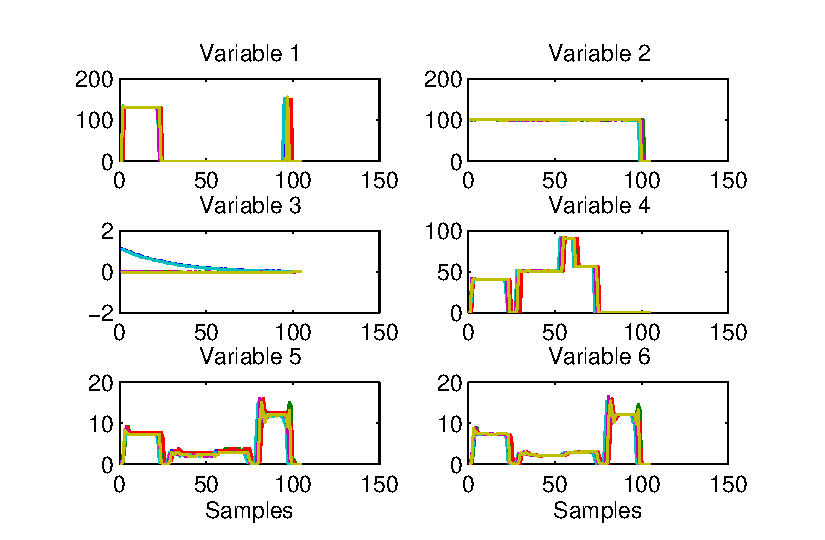
\includegraphics[width=0.45\textwidth]{figures/application/fig_raw_data_1.eps}
    \label{fig:raw_data_1}
}
\subfigure[]{
  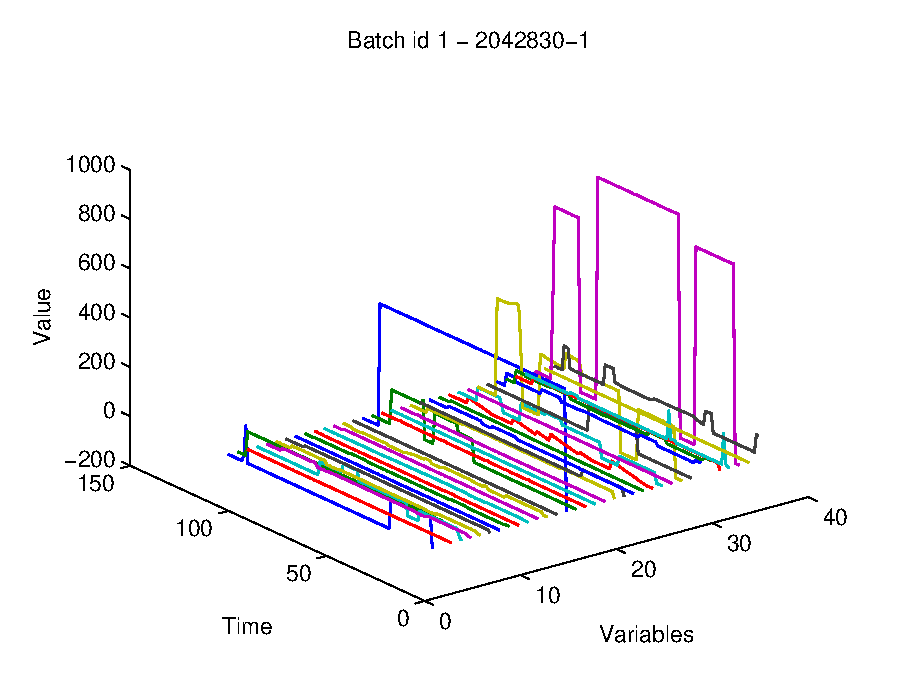
\includegraphics[width=0.45\textwidth]{figures/application/fig_raw_data_2.eps}
    \label{fig:raw_data_2}

} \subfigure[]{
  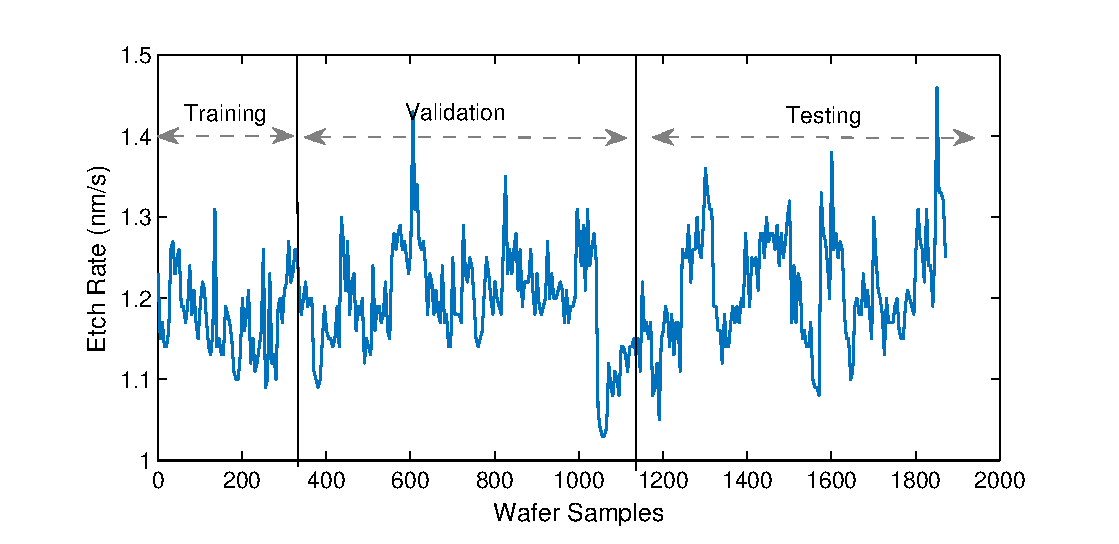
\includegraphics[width=0.95\textwidth]{figures/application/fig1_output_raw.eps}
    \label{fig:raw_data_3}
} \caption[raw data plot]{Raw data plot showing \subref{fig:raw_data_1} the
temporal profiles of six variables for five wafer batches,
\subref{fig:raw_data_2} A three-dimensional representation of trajectories
from a single batch, and \subref{fig:raw_data_3} output variable etch rate}
\label{fig:raw_data}
\end{figure}

\clearpage
\subsection{Data Pretreatment}
Missing and redundant data, empty rows and columns are first removed from the dataset. 
Temporal outliers such as spikes in sensor readings were also removed.
After initial cleaning, the dataset was then unfolded into a 2-D array using
batch-wise unfolding \cite{Westerhuis1999}. Batch-wise outliers were then removed from the unfolded data. Additional data sanitation checks utilizing process knowledge were also carried out. For example, batches where there are significant trajectory deviations in the recipe step were removed. After initial trajectory screening, the trajectories were then aligned using
robust-derivative dynamic time warping \cite{Zhang2013} based on the
indicator variable ``recipe number''. Univariate scaling and mean-centering
were then applied to the unfolded input-output data to create the
$\mathbf{X}$ and $\mathbf Y$ matrices.


\subsection{GSMMS with PLS local model}
A GSMMS model with local PLS models was trained for this data
set. The resulting unfolded multi-way dataset contains approximately 650
inputs. 
The feature input into the GSOM consisted of the first three principal component scores of the PCA projection of the unfolded training data. 
Initial offline batch training produced a 5 node GSOM network; its network structure and the feature inputs (first two PCA scores) are plotted in Figure~\ref{fig:gate_etch_gsmms_training}.
The scores show a parabolic shape for the training inputs, indicating that there is strong non-steady-state operation in the process. 

To simulate online adaptation, the GSMMS model was updated batch-wise for every five wafers. The most recent GSMMS model was used for prediction (from 1-step ahead to 5 step-ahead). The resulting network structure after iterating through the entire testing data is shown in
Figure~\ref{fig:gate_etch_gsmms_testing}. Comparing against the offline trained GSOM, the network size has increased to 6 nodes. We also observe an increased density of nodes around the left
``tail'' of the parabola. This indicates that particular region had higher activation rates in the more recent data. The prediction performance of the adaptive GSMMS is plotted in
Figure~\ref{fig:gate_etch_gsmms_prediction}. The adaptive GSMMS was able to successfully track the measured etch rate across two maintenance events (around sample 220 and sample 800). The GSMMS performance was also compared against several benchmark methods in Table~\ref{tbl:final_comparison}.


\begin{figure}[!htpb]
  \centering
    \subfigure[]{
    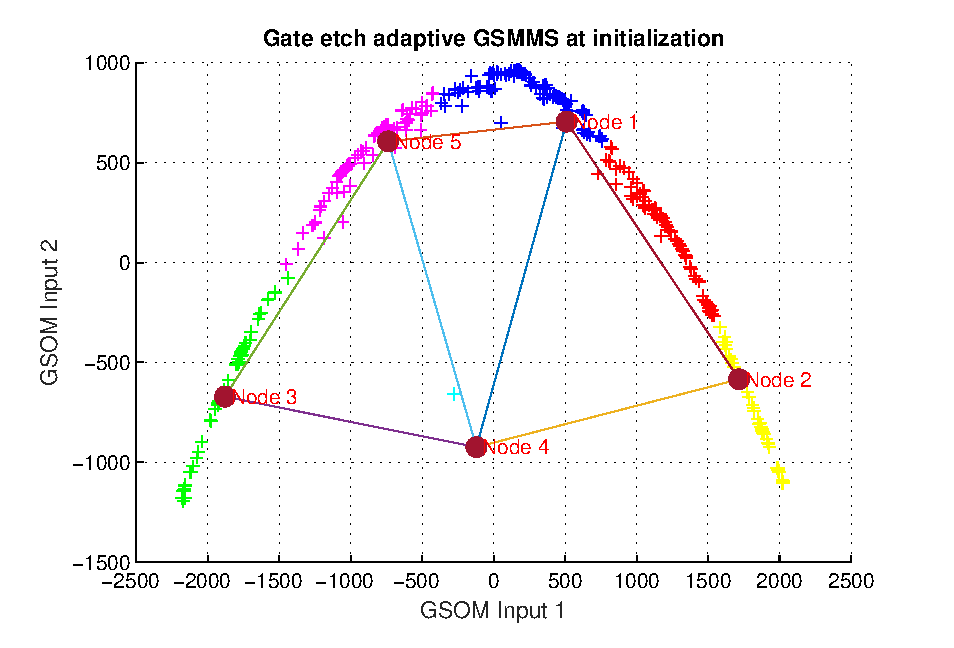
\includegraphics[width=0.45\textwidth]{figures/application/gate_etch_gsmms_training.eps}
    \label{fig:gate_etch_gsmms_training}
    }
  \subfigure[]{
    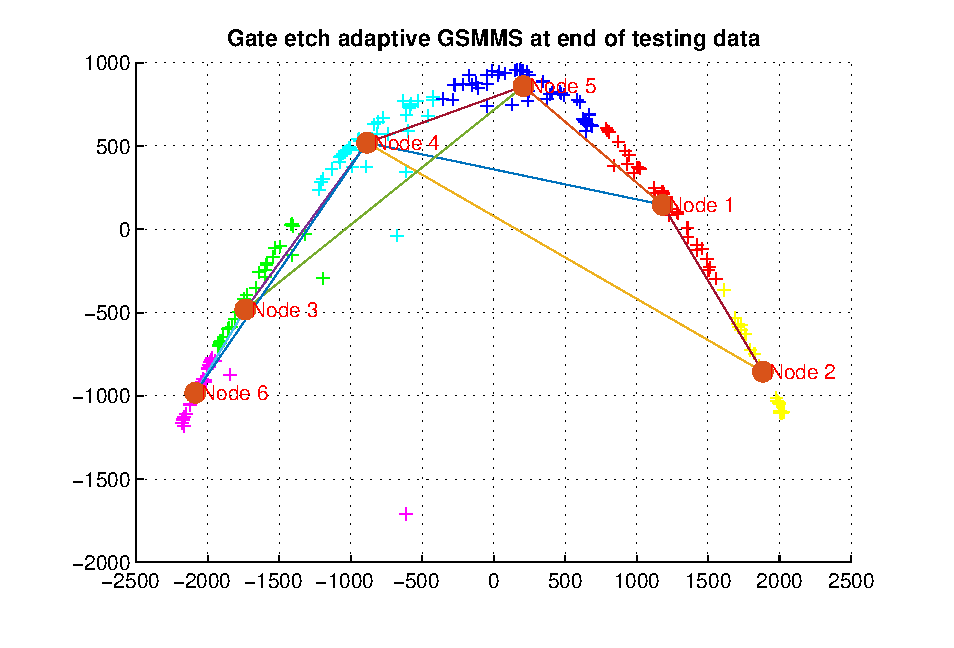
\includegraphics[width=0.45\textwidth]{figures/application/gate_etch_gsmms_testing.eps}
    \label{fig:gate_etch_gsmms_testing}
    }
  \caption{Gate Etch adaptive GSMMS \subref{fig:gate_etch_gsmms_training} post-training and \subref{fig:gate_etch_gsmms_testing} final (after testing data update) network structure}\label{fig:gate_etch_gsmms}
\end{figure}

\begin{figure}
  \centering
  % Requires \usepackage{graphicx}
  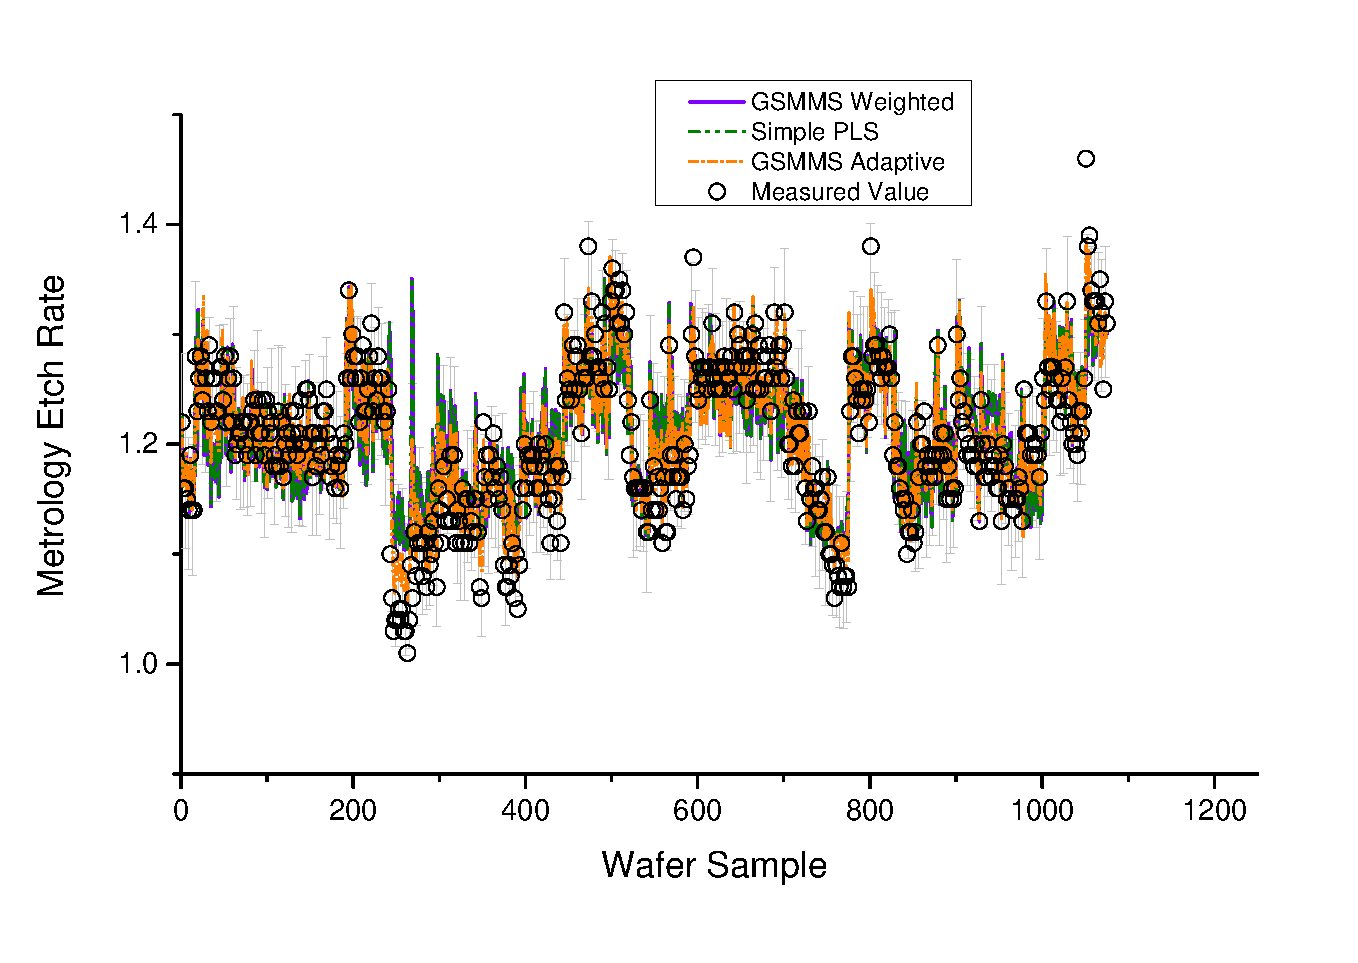
\includegraphics[width=0.95\textwidth]{figures/application/gate_etch_gsmms_prediction.eps}\\
  \caption{Prediction results of the Adaptive GSMMS model for the testing dataset}\label{fig:gate_etch_gsmms_prediction}
\end{figure}

\clearpage

\begin{table}[htpb]
\centering
\caption {Model size, coefficient of determination, and cross-validated root mean squared residual of candidate models}
\footnotesize
    \begin{tabular}{lccc}
    \toprule
       Method                               &    Approx. model size &  Testing $R^2$ & RMS residual \\ \hline
       PCA regression &    2700          & 0.425               & 0.0495     \\
       BPNN    &       $2700\times N_{layers}$    & 0.72 / 0.32 &  0.0823 \\
       Nonlinear PLS with Neural networks & $600 \times A \times N_{layers}$ & 0.56 / 0.25                          & 0.0623      \\
       Static PLS &    600          & 0.142              & 0.0998     \\ \hline
       MW-PLS &    600          & 0.442              & 0.0598     \\
       MW-PLS w/ TPLS&    ~600          & 0.66              & 0.029     \\
       Adaptive GSMMS-PLS &    $600 \times 5\rightarrow 600 \times 6 $          & 0.812              & 0.019     \\
       \bottomrule
    \end{tabular}
    \label{tbl:final_comparison}
\end{table}

\begin{table}[htpb]
\centering
\caption {Qualitative evaluation of the candidate models and their implementation difficulty}
    \label{tbl:final_comparison2}
\footnotesize
\resizebox{\textwidth}{!}{
    \begin{tabular}{lccc p{2cm}}
    \toprule
       Method               &    \parbox{2cm}{Development Difficulty} & Prediction $R^2$ &  Implementation Difficulty\\ \hline
       PCA regression       &      Easy              &     0.2-0.5      &       \parbox{4.5cm}{ Medium (large memory requirement)} \\
       Static PLS           &      Easy              &     0.1-0.5      &      \parbox{4.5cm}{  Easy           }    \\
       BPNN                 &  Medium                &    0-0.7         &      \parbox{4.5cm}{ Difficult(nonlinear activation function)           } \\
       Nonlinear PLS        &  Medium                &    0-0.7         &     \parbox{4.5cm}{Difficult (nonlinear + large memory requirement)  }           \\ \hline
       MW-PLS               &    Easy                &    0.2-0.6        &     \parbox{4.5cm}{Difficult (requires online update)          } \\
       MW-PLS w/ TPLS       &    Medium               &    0.5-0.6         &      \parbox{4.5cm}{   Difficult  (requires online update and filtering logic)    } \\
       Adaptive GSMMS-PLS   &    Difficult          &     0.6-0.8         &      \parbox{4.5cm}{Difficult (requires online update and computationally expensive)} \\
       \bottomrule
    \end{tabular}
}
\end{table}

\clearpage

\subsection{Comparison with other techniques}

The model size, prediction error, and $R^2$ value of GSMMS, Principal component regression (PCA regression), PLS, Back-propagated Neural Network (BPNN), nonlinear PLS using neural networks (NN-PLS), and moving window PLS are listed in Table~\ref{tbl:final_comparison}.

%Principal component regression (PCA), back-propagated neural network (BPNN) ,
%neural network PLS (NNPLS), and moving window partial least squares without
%TPLS detection (MW-PLS) were implemented on the same dataset to compare the
%results with our proposed framework. Table \ref{tbl:final_comparison} lists
%the comparison results; the three metrics used to evaluate model performances
%are parameter size, cross-validated coefficient of determination ($R^2$), and
%cross validated root mean squared prediction error (RMSPECV).

The PCA regression model used the full dataset (without
variable filtering) and was found to be the most effective with 10
components. The back-propagated neural network model used the same reduced set of
unfolded inputs as the GSMMS (650 inputs). A two-layer structure
with 10 neurons in the first layer was chosen. This network configuration resulted in 6210 weights in the BPNN model. While the training score was very good, performance degradation towards later part of the testing data was observed. The
testing $R^2$ in the BPNN model was around 0.72 for about 200 wafers
initially, but it decreased quickly to around 0.32 afterwards. For NN-PLS, 10
outer components was used. The inner neural network size varied between 3 to
6, and was trained using the Levenberg-Marquadt back-propagation. The NN-PLS
was able to provide reasonable approximation initially but also experienced
relatively fast degradation in performance similar to BPNN; the drop in
performance indicate that static methods could not model the process drift. The PLS
with moving window (MW-PLS) update also used the same set of inputs to ensure comparison consistency. However, just applying MW-PLS directly was ineffective due to outliers and abnormal
runs in testing data. Using the MW-PLS with TPLS outlier removal approach resulted in much better prediction performance \cite{Lu2014a}. The GSMMS model gave the best prediction
performance among the adaptive techniques (MW-PLS and MW-PLS w/ TPLS).
However, GSMMS model is also more complex in model structure.

In any practical industrial system, it is also important to consider
the development and maintenance costs of a solution. Table~\ref{tbl:final_comparison2} lists the qualitative assessment of total costs of the models and methods in terms of their development
difficulty, deployment difficulty, and modeling performance. These metrics
were assessed subjectively based on our experiences. In general, static methods such as the PCA regression or PLS regression are preferred for their simplicity. However, in cases where discontinuity and process degradation strongly affect the model performance, more advanced techniques such as GSMMS can be applied to further improve the performance.
